% stura-voting-doc (c) by Fabian Wenzelmann
%
% stura-voting-doc is licensed under a
% Creative Commons Attribution 4.0 International License.
%
% You should have received a copy of the license along with this
% work. If not, see <http://creativecommons.org/licenses/by/4.0/>.

\chapter{Abstimmungsperioden und Abstimmungsberechtigte}
\section*{Abstimmungsperioden}
Eine Abstimmungsperiode ist die gröbste Einteilung von Sitzungen.
Eine Periode beschreibt in unserem Fall ein Semester, z.B. das Sommersemester
2019.

Eine neue Periode kann über das \emph{Hauptmenü} angelegt werden.
Das Hauptmenü ist in Abbildung \ref{fig:main-menu} dargestellt.
Unter \emph{Neu} $\rightarrow$ \emph{Sitzungsperiode} kann eine neue Periode
erstellt werden.
Eine Abstimmungsperiode hat einen Start- und Endzeitpunkt (normalerweise
Semesteranfang und Semesterende).
Zudem kann hier gleich eine Revision (nächster Abschnitt) angelegt werden.

\begin{figure}
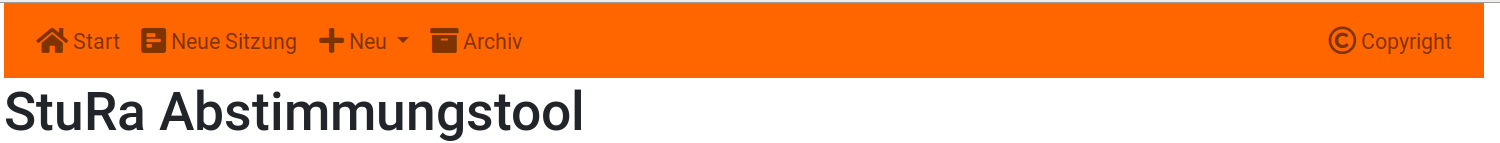
\includegraphics[width=\textwidth]{../images/main_menu}
\caption{Das Hauptmenü}
\label{fig:main-menu}
\end{figure}

\section*{Revisionen}
Für eine Sitzung benötigen wir natürlich eine Liste aller abstimmungsberechtigten
Gruppen (Fachbereiche und Initiativen).
Während dem Semester können sich dabei durchaus Dinge an dieser Liste verändern:
Eine Gruppe verliert ihr Stimmrecht, das Stimmgewicht der Gruppe muss angepasst
werden etc.

Eine solche Zusammenfassung bezeichnen wir als \emph{Revision}.
Eine solche Revision ist immer einer Abstimmungsperiode zugeordnet.
Angelegt werden kann diese über das Hauptmenü \emph{Neu} $\rightarrow$
\emph{Revision}.
Hier wählt man das entsprechende Semester aus der Liste aus.
Zusätzlich kann man noch eine Notiz anlegen, z.B. ``Fachbereich XY hat Stimmberechtigung verloren''.

Die Abstimmungsberechtigen werden zeilenweise nach folgender Syntax erstellt:

\texttt{* <NAME>: <GEWICHT>}.
Angenommen es gibt die folgenden Abstimmungsberechtigten

\begin{center}
\begin{tabular}{@{}ll@{}}
\toprule
  Name & Gewicht\\ \midrule
  Fachbereich Foo & 3 \\
  Fachbereich Bar & 2 \\
  Initiative XY & 1 \\
\bottomrule
\end{tabular}
\end{center}

Dann trägt man folgendes in das Feld ein:

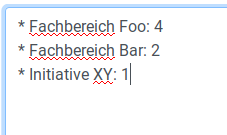
\includegraphics{../images/voters_revision}

\section*{Anzeigen und Bearbeiten}
Eine Liste aller Abstimmungsperioden ist über das Archiv verfügbar.
Klickt man eine Abstimmungsperiode an sieht, man eine Liste aller
Revisionen die zu dieser Periode gehören.
Sowohl Abstimmungsperioden als auch Revsionen haben einen \emph{Bearbeiten}
Button.
Hier lassen sich bestimmte Einstellungen ändern.
\begin{importantbox}{Achtung}
Es ist möglich, die Stimmgewichte einer Revision bearbeiten.
Dies sollte man aber nur im äußersten Notfall tun!
Wenn sich etwas an den bisherigen Gewichten ändert oder eine Gruppe nicht mehr
abstimmungsberechtigt ist, sollte eine neue Revision angelegt werden.
Alle mit dieser Revision durchgeführten Abstimmungen verändern sich!
Der einzige Zeitpunkt an dem eine Revision geändert werden sollte ist direkt
nach dem Erstellen (wenn es noch keine Abstimmung gibt).
\end{importantbox}
Der Grund ist, dass alle Sitzungen und Abstimmungen mit einer bestimmten Revision
verknüpft sind.
Ändert sich nun diese Revision kann dies auch Abstimmungsergebnisse ändern.
Deshalb sollte man immer eine neue Revision anlegen.
Der entsprechende Hinweis wird auch auf der Bearbeiten Seite angezeigt.

Zudem verfügen beide Ansichten über \emph{Löschen} Buttons.
Auch hier muss man aufpassen:
\begin{importantbox}{Achtung}
Löscht man eine Abstimmungsperiode werden alle dazugehörigen Revisionen und
Sitzungen ebenfalls gelöscht.
Löscht man eine Revision werden alle zu dieser Revision gehörenden Sitzungen
gelöscht.

Dies beinhaltet sowohl die eigentlichen Abstimmungen als auch die Ergebnisse
der Abstimmungen.
\end{importantbox}
